\documentclass[12pt, a4paper, oneside]{article}
\usepackage[utf8]{inputenc}
\usepackage[T1]{fontenc}
\usepackage[english]{babel}
\usepackage[left=2cm,right=2cm,top=2cm,bottom=2cm]{geometry}
\usepackage{listings}
\usepackage{placeins}
\usepackage{graphicx}

\usepackage[
  backend=biber,
  style=authoryear-icomp,
  sortlocale=en_US,
  natbib=true,
  url=true, 
  doi=true,
  eprint=false
]{biblatex}

\usepackage[capposition=top]{floatrow}

\usepackage{xcolor}
\usepackage{varioref}
\usepackage{hyperref}
\usepackage{cleveref}

\hypersetup{
  colorlinks=true,
}
\addbibresource{bibliography.bib}

\title{AIND: Mimic Me!}
\author{Markus Mayer}
\date{\today}

\begin{document}

\maketitle

\begin{abstract}
  This project implements a simple face tracking and emotion detection demo using 
  the Affectiva Emotion AI SDK \cite{affectiva}. 
  Each face is tagged with an appropriate emoji next to it and small game is implemented
  where the player needs to mimic a random emoji displayed by the computer.
\end{abstract}

 \begin{figure}[!h]
  \centering
  
\includegraphics[width=10cm]{images/laughing}
  \caption{Detected facial features and dominant emoji}
  \label{fig:laughing}
 \end{figure}

\section{Multi-face feature detection}

The original code was modified to display results for multiple detected faces.
However, during testing only one detected face was returned by the API.

\section{Rendering the feature points}

For each detected face, a list coordinates for defined feature points is returned.
The points are rendered as transparent overlays at the reported coordinates in the webcam image (\cref{fig:laughing}).

\section{Showing the dominant Emoji}

Similar to the feature points, a set of defined emotions and their according emoji is returned,
where the dominant emoji is reported back as a unicode string.
The location of feature point $10$ is used to pin a rendered emoji to the left eyebrow of
each detected face (\cref{fig:laughing}).

\section{Mimic Me!}

A small game dubbed "Mimic Me" was implemented where the players need to match their
facial expression to a presented Emoji (\cref{fig:screenshot}).
Multiple players are supported (if multiple faces are returned from the API \cite{affectiva:analyze}),
however playing is cooperative.
Since the API sometimes returned wrong results (probably due to my beard), I addeda a skip button 
to select a new Emoji without having to reset the game.
No timeout is implemented and playing is basically forever.

\begin{figure}
  \centering
  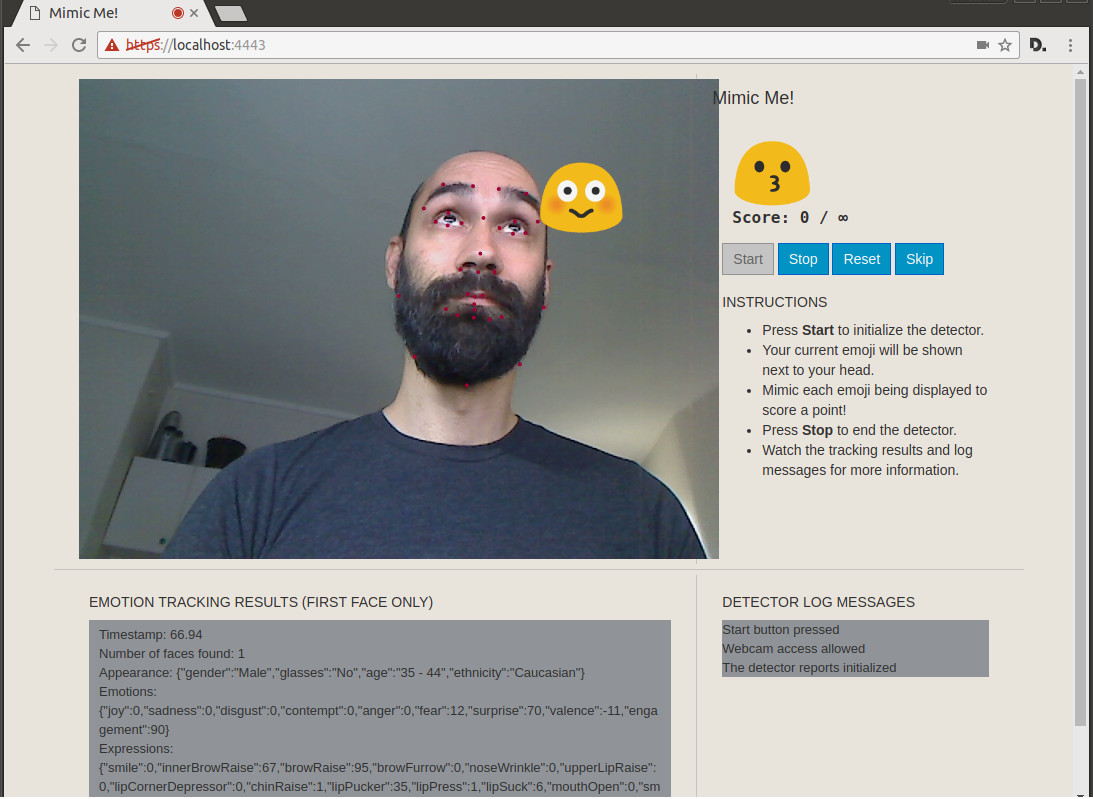
\includegraphics[width=\textwidth]{images/page}
  \caption{A screenshot of the demo}
  \label{fig:screenshot}
 \end{figure}

 \printbibliography 

\end{document}
